Our FPGA design for convolutional neural networks is an attempt to decrese the cost per iteration of training a CNN. While it does use some techniques that may change the convergence of the neural network, algorithmically, it is serially equivalent to software implementations for training a CNN. This is important, because we are not trying to create a new parallelized algorithm such as {\sc{Hogwild!}}, we are only trying to apply traditional hardware speed-up techniques to CNNs.

Currently, most of the computation cost of a CNN is concentrated in the convolutional layers. Furthermore, attempts at hardware parallelization have been hampered by the cost of memory accesses. In order to tackle these issues, we designed a fundamental \textit{convolutional filter unit}. Each filter unit represents a single convolutional filter in a CNN, and each layer of a CNN can contain several convolutional filters. We wanted to run these filters in parallel, so that we only pay the cost of sliding the filter over the entire input image space once per layer. Thus, we needed to keep the resource cost of each filter low enough that multiple filter units can be instantiated in the hardware. To do this, we use 16-bit fixed point (14 fractional bits, 1 sign bit) hardware with stochastic quantization throughout the FPGA implementation \cite{limited-precision}. Stochastic rounding or quantization is described by Eq. \ref{eq:stochastic-rounding-def} where $\epsilon$ is machine epsilon (i.e. machine precision) for a given fixed point system.
\begin{equation}
	\mathrm{Round}(x) = \begin{cases}
		\lfloor x \rfloor & \quad \text{with probability } 1 - \frac{x - \lfloor x \rfloor}{\epsilon} \\
		\lfloor x \rfloor + \epsilon & \quad \text{with probability } \frac{x - \lfloor x \rfloor}{\epsilon}
	\end{cases}
	\label{eq:stochastic-rounding-def}
\end{equation}
Gupta et al. describe how to implement such a rounding mechanism in hardware in the presentations accompanying their paper \cite{limited-precision}. Fig. \ref{fig:stochastic-quantizer-block-diagram} rounds a higher precision number by adding to the lower (discarded) fractional bits, as is common in round-to-nearest quantization schemes. However, stochastic rounding adds a pseudorandom number to the lower bits instead of pre-determined number. The pseudorandom number is generated using a linear feedback shift register (LFSR) as detailed in Fig. \ref{fig:lfsr-block-diagram}.
\begin{figure}[ht]
	\centering
	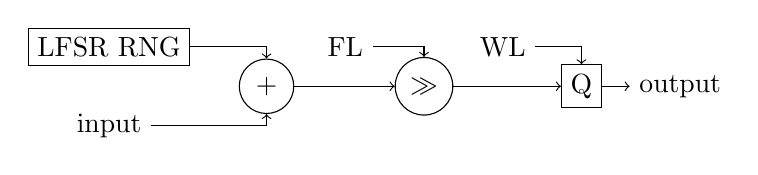
\begin{tikzpicture}
		\node (input) at (0, 0) {input};
		\node [draw, rectangle] (lfsr) at (0, 1) {LFSR RNG};

		\node [draw, circle] (add) at (2, 0.5) {$+$};
		\draw [->] (lfsr.east) -| (add.north);
		\draw [->] (input.east) -| (add.south);

		\node [draw, circle] (shift) at (4, 0.5) {$\gg$};
		\node (shift-val) at (3, 1) {FL};
		\draw [->] (add.east) -- (shift.west);
		\draw [->] (shift-val.east) -| (shift.north);

		\node [draw, rectangle] (quantizer) at (6, 0.5) {Q};
		\node (quantizer-val) at (5, 1) {WL};
		\draw [->] (shift.east) -- (quantizer.west);
		\draw [->] (quantizer-val.east) -| (quantizer.north);

		\draw [->] (quantizer.east) -- ++(10pt, 0) node [right] (output) {output};
	\end{tikzpicture}
	\caption{Stochastic rounding quantizer (FL is fractional length; WL is word length; Q selects the WL LSBs of its input)}
	\label{fig:stochastic-quantizer-block-diagram}
\end{figure}
\begin{figure}[ht]
	\centering
	\begin{tikzpicture}[circuit logic US]
		\draw (0, 0) rectangle (8, 0.5);
		\foreach \i in {1, ..., 15} {
			\draw (0.5*\i, 0) -- (0.5*\i, 0.5);
		}
		\foreach \i in {0, ..., 15} {
			\node (bit\i) at (0.5*\i + 0.25, 0.25) {\i};
		}

		\node [xor gate, point left, inputs={nn}] (xor1) at (6, 2) {};
		\draw (bit15.north) |- (xor1.input 2);
		\draw (bit13.north) |- (xor1.input 1);

		\node [xor gate, point left, inputs={nn}] (xor2) at (5, 1.5) {};
		\draw (xor1.output) |- (xor2.input 2);
		\draw (bit12.north) |- (xor2.input 1);

		\node [xor gate, point left, inputs={nn}] (xor3) at (4, 1) {};
		\draw (xor2.output) |- (xor3.input 2);
		\draw (bit10.north) |- (xor3.input 1);

		\draw (xor3.output) -- ++(-4, 0) |- (bit0.west);
	\end{tikzpicture}
	\caption{16-bit linear feedback shift register}
	\label{fig:lfsr-block-diagram}
\end{figure}
In addition to reducing the hardware resources required to perform arithmetic operations, using 16-bit fixed point numbers significantly reduces the computation time of an adder or multiplier, and it reduces the memory footprint required to store numbers. These benefits will be important when we discuss the design of each filter unit.

In addition to using fixed point numbers to speed up computation, we exploit spatial locality and operational level parallelism when design the filter units. Each unit contains its own register file to store the weights and biases related to it. This way, the weight and bias vectors do not need to be fetched or stored in memory, and they do not need to be passed around. As a result, the filter unit is capable of not only computing the feed-forward pass for each training sample, but also propagating error back through the network and using the error to compute gradients and update its own weights. Lastly, the major operation performed by a filter unit is a vector dot product. This involves a series of multiplications and additions. The multiplications are performed in parallel, and the additions use a binary tree-like structure to perform as many additions in parallel as possible. For an $n \times 1$ vector, our addition structure takes $\log(n) \cdot d$ delay (where $d$ is the delay for a single addition), while a naive implementation takes $(n - 1) \cdot d$ time. Fig. \ref{fig:conv-filter-module} illustrates a block level diagram of a filter unit (though the diagram includes some control signals, it does not include all of them to save space).
\begin{figure}[ht]
	\centering
	\begin{tikzpicture}
		\foreach \i in {0, ..., 4} {
			\node (in1\i) at (0, -2*\i) {in1$_\i$};
		}

		\draw (0, 3) node[above right] {Weight Register File} rectangle (2, 1.75);
		\foreach \i in {0, ..., 4} {
			\draw ($(0, {2.75-0.25*\i})$) node[above] (wrf\i) {} --++ (2, 0) node[above] (wrf\i-out) {};
		}

		\foreach \i in {0, ..., 4} {
			\node[circle, draw] (mul\i) at ($(3+0.5*\i, -2*\i)$) {$\times$};
			\node[multiplexer, rotate=270] (mux\i) at ($(3+0.5*\i, -2*\i + 0.8)$) {};
			\draw [->] (in1\i) -- (mul\i.west);
			\draw [->] (wrf\i-out) -| (mux\i.north west);
			\draw [<-] (mux\i.south west) --++ (0, 10pt) --++ (-10pt, 0) node [left] (in2\i) {in2$_\i$};
			\draw [->] (mux\i.east) -- (mul\i.north);
			\draw (mux\i.south) --++ (-10pt, 0) node [left] {$s$};
		}

		\node[circle, draw] (dot-product-sum) at (7, -4) {$+$};

		\foreach \i in {0, ..., 4} {
			\pgfmathtruncatemacro{\angle}{90 + 45*\i};
			\draw [->] (mul\i.east) --++ ($(2.5 - 0.5*\i, 0)$) -- (dot-product-sum.\angle);
		}

		\node[rectangle, minimum height=0.5cm, minimum width=0.5cm, draw] (dot-product-quantizer) at (8.5, -4) {Q};
		\draw [->] (dot-product-sum) --++ (0.75, 0) node (fb) {} -- (dot-product-quantizer);
		\draw [->] (fb.center) --++ (0, 15pt) -- (dot-product-sum.45);

		\node[circle, draw] (bias-sum) at (10, -4) {$+$};
		\draw [->] (dot-product-quantizer) -- (bias-sum);
		\draw (9, -3.25) rectangle ++ (2, 0.25);
		\node at (10, -2.75) {Bias Register File};
		\draw [->] (10, -3.25) -- (bias-sum.north);

		\node[rectangle, minimum height=0.5cm, minimum width=0.5cm, draw] (sigma-prime) at (12, -3) {$\sigma'$};
		\node[rectangle, minimum height=0.5cm, minimum width=0.5cm, draw] (sigma) at (12, -5) {$\sigma$};
		\draw [<-] (sigma-prime.west) --++ (-5pt, 0) -- (bias-sum.30);
		\draw [<-] (sigma.west) --++ (-5pt, 0) -- (bias-sum.330);

		\node [circle, draw] (act-der-mul) at (8.5, -5.65) {$\times$};
		\draw [->] (dot-product-quantizer.south) -- (act-der-mul);
		\draw [<-] (act-der-mul.south) --++ (0, -10pt) node [below] {Activation Derivative};

		\node[multiplexer] (out2-mux) at (13, -3.325) {};
		\draw [->] (sigma-prime.east) -- (out2-mux.north west);
		\draw [<-] (out2-mux.south west) --++ (-10pt, 0) node [left] {0};
		\draw (out2-mux.south) --++ (0, -10pt) node [below] {$s$};
		\draw [->] (out2-mux.east) --++ (10pt, 0) node [right] {out2};

		\node[multiplexer] (out1-mux) at (13, -5.325) {};
		\draw [->] (sigma.east) -- (out1-mux.north west);
		\draw [->] (act-der-mul) -- (out1-mux.south west);
		\draw (out1-mux.south) --++ (0, -10pt) node [below] {$s$};
		\draw [->] (out1-mux.east) --++ (10pt, 0) node [right] {out1};

		\node[circle,draw] (grad-mul) at (8.5, -1) {$\times$};
		\draw [->] (dot-product-quantizer.north) -- (grad-mul.south);
		\draw [<-] (grad-mul.west) --++ (-10pt, 0) node [left] {$\gamma$};
		\draw [->] (grad-mul.east) --++ (10pt, 0) node [right] {Gradient Update};

		\draw (6.5, 3) rectangle (12.5, 0);
		\node [align=left] at (9.5, 1.5) {If $s = $ Gradient Update Mode,\\then Weights -= Gradient Update\\and Bias -= sum(in2) (not shown)};
	\end{tikzpicture}
	\caption{A convolutional layer filter unit}
	\label{fig:conv-filter-module}
\end{figure}

Though Fig. \ref{fig:conv-filter-module} illustrates a $5 \times 1$ vector of inputs and weights, our implementation uses a $3 \times 3$ patch which results in $9 \times 1$ vector of inputs. During a feed-forward pass, the filter unit is fed with a patch of inputs. An input contains a 3D tensor, but each patch is only 2D. Control signals are used to inform the filter unit which slice of inputs along the third dimension it is operating on. Accordingly, it fetches the correct inputs performs the dot product. An accumulator register stores the output of successive dot products as patches along the third dimension are supplied to the filter unit. After traversing across the depth dimension, the filter unit quantizes the result of the dot product and adds the bias. This result is passed through $\sigma$ and $\sigma'$. The $\sigma$ output is a single pixel of output from the layer, and the $\sigma'$ is stored for later use.

During the feed-backward pass, the filter unit first propagates the error by convolving the rotated weight kernel with the error from the previous layer. It is provided with the previously stored $\sigma'$ values through the activation derivative input. The output of this step is stored pixel by pixel as the error for the convolutional layer.

The next stage is the gradient update stage. The filter unit is provided with the appropriate input map and error map to compute the gradient for the appropriate subset of the weight kernel. The error patches are also accumulated using a binary tree adder structure and an accumulator register. This result is the gradient update for the bias. After performing the convolution and accumulation operations, the gradients are used to update the bias and weight values.

On a higher level, we perform convolution by first accumulating across the depth dimension, then sliding across horizontal and vertical directions. We perform max pooling by sliding a pooling filter across the input horizontal and vertical directions. Across the depth dimension, max pooling is done in parallel. The fully-connected layer is done on $16 \times 1$ patches of vectors at a time. But the fully-connected patch operation is performed in parallel for all 10 output elements.